%\documentclass{article}
%\usepackage{graphicx,subfigure}
%\begin{document}

\begin{figure}[h]
  \centering
   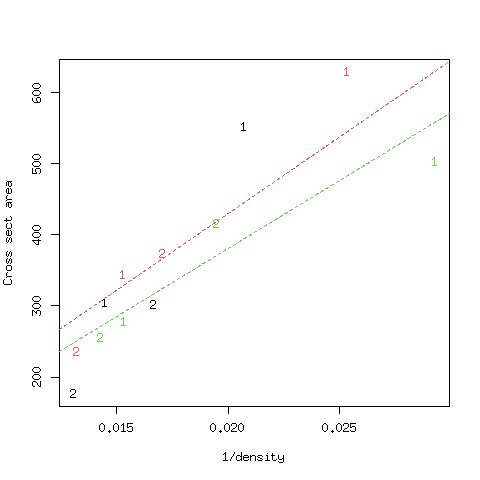
\includegraphics[width=0.9\textwidth]{C19391951/strainxnut.png}
  \caption{Plot of breed means for reciprocal of follicle density and fibre cross sectional area from Carter(1939)~\cite{cart:39}. The red line is a linear regressions  with zero intercept fitted to strain x age means for the high nutrition group. The green line is a linear regressions with zero intercept fitted to strain x age means for the Low nutrition group.}
  \label{fig:oldcart1}
\end{figure}

%\end{document}

